\documentclass[12pt,twoside]{report}

%%%%%%%%%%%%%%%%%%%%%%%%%%%%%%%%%%%%%%%%%%%%%%%%%%%%%%%%%%%%%%%%%%%%%%%%%%%%%

% Definitions for the title page
% Edit these to provide the correct information

\newcommand{\reporttitle}{Detección de anomalías}
\newcommand{\reportauthor}{David Alberto Martín Vela}
\newcommand{\subject}{Inteligencia de Negocio}
\newcommand{\degreetype}{Doble Grado Ingeniería Informática y Matemáticas}
\newcommand{\email}{\href{mailto:davidmv1996@correo.ugr.es}{davidmv1996@correo.ugr.es}}

%%%%%%%%%%%%%%%%%%%%%%%%%%%%%%%%%%%%%%%%%%%%%%%%%%%%%%%%%%%%%%%%%%%%%%%%%%%%%

% load some definitions and default packages
%%%%%%%%%%%%%%%%%%%%%%%%%%%%%%%%%%%%%%%%%
% University Assignment Title Page 
% LaTeX Template
% Version 1.0 (27/12/12)
%
% This template has been downloaded from:
% http://www.LaTeXTemplates.com
%
% Original author:
% WikiBooks (http://en.wikibooks.org/wiki/LaTeX/Title_Creation)
%
% License:
% CC BY-NC-SA 3.0 (http://creativecommons.org/licenses/by-nc-sa/3.0/)
% 
%
%%%%%%%%%%%%%%%%%%%%%%%%%%%%%%%%%%%%%%%%%
%----------------------------------------------------------------------------------------
%	PACKAGES AND OTHER DOCUMENT CONFIGURATIONS
%----------------------------------------------------------------------------------------
\usepackage[a4paper,hmargin=2.8cm,vmargin=2.0cm,includeheadfoot]{geometry}
\usepackage{textpos}
\usepackage{tabularx,longtable,multirow,subfigure,caption}%hangcaption
\usepackage{fncylab} %formatting of labels
\usepackage{fancyhdr} % page layout
\usepackage{url} % URLs
\usepackage[english]{babel}
\usepackage{amsmath}
\usepackage{graphicx}
\usepackage{dsfont}
\usepackage{epstopdf} % automatically replace .eps with .pdf in graphics
\usepackage{array}
\usepackage{latexsym}
\usepackage{booktabs}
\usepackage[pdftex,hypertexnames=false,colorlinks]{hyperref} % provide links in pdf
\usepackage[
    type={CC},
    modifier={by-nc-sa},
    version={3.0},
]{doclicense}
\usepackage[
backend=bibtex,
style=alphabetic,
sorting=ynt
]{biblatex}
\addbibresource{refs.bib}

\usepackage{listings}
\usepackage{color}
\usepackage{multicol}
\definecolor{dkgreen}{rgb}{0,0.6,0}
\definecolor{gray}{rgb}{0.5,0.5,0.5}
\definecolor{mauve}{rgb}{0.58,0,0.82}

\lstset{frame=tb,
  language=R,
  aboveskip=0.5mm,
  belowskip=0.5mm,
  showstringspaces=false,
  columns=flexible,
  basicstyle={\small\ttfamily},
  numbers=none,
  numberstyle=\tiny\color{gray},
  keywordstyle=\color{blue},
  commentstyle=\color{dkgreen},
  stringstyle=\color{mauve},
  breaklines=true,
  breakatwhitespace=true,
  tabsize=1
}

\hypersetup{pdftitle={},
  pdfsubject={}, 
  pdfauthor={},
  pdfkeywords={}, 
  pdfstartview=FitH,
  pdfpagemode={UseOutlines},% None, FullScreen, UseOutlines
  bookmarksnumbered=true, bookmarksopen=true, colorlinks,
    citecolor=black,%
    filecolor=black,%
    linkcolor=black,%
    urlcolor=black}

\usepackage[all]{hypcap}


%\usepackage{color}
%\usepackage[tight,ugly]{units}
\usepackage{float}
%\usepackage{tcolorbox}
%\usepackage[colorinlistoftodos]{todonotes}
% \usepackage{ntheorem}
% \theoremstyle{break}
% \newtheorem{lemma}{Lemma}
% \newtheorem{theorem}{Theorem}
% \newtheorem{remark}{Remark}
% \newtheorem{definition}{Definition}
% \newtheorem{proof}{Proof}


%%% Default fonts
\renewcommand*{\rmdefault}{bch}
\renewcommand*{\ttdefault}{cmtt}
\renewcommand{\contentsname}{Índice}

%%% Default settings (page layout)
\setlength{\parindent}{0em}  % indentation of paragraph

\setlength{\headheight}{14.5pt}
\pagestyle{fancy}
\renewcommand{\chaptermark}[1]{\markboth{\chaptername\ \thechapter.\ #1}{}} 

\fancyfoot[ER,OL]{\sffamily\textbf{\thepage}}%Page no. in the left on odd pages and on right on even pages
\fancyfoot[OC,EC]{\sffamily }
\renewcommand{\headrulewidth}{0.1pt}
\renewcommand{\footrulewidth}{0.1pt}
\captionsetup{margin=10pt,font=small,labelfont=bf}


%--- chapter heading

\def\@makechapterhead#1{%
  \vspace*{10\p@}%
  {\parindent \z@ \raggedright \sffamily
    \interlinepenalty\@M
    \Huge\bfseries \thechapter \space\space #1\par\nobreak
    \vskip 30\p@
  }}

%---chapter heading for \chapter*  
\def\@makeschapterhead#1{%
  \vspace*{10\p@}%
  {\parindent \z@ \raggedright
    \sffamily
    \interlinepenalty\@M
    \Huge \bfseries  #1\par\nobreak
    \vskip 30\p@
  }}

\allowdisplaybreaks

% load some macros
% Here, you can define your own macros. Some examples are given below.

\newcommand{\R}[0]{\mathds{R}} % real numbers
\newcommand{\Z}[0]{\mathds{Z}} % integers
\newcommand{\N}[0]{\mathds{N}} % natural numbers
\newcommand{\C}[0]{\mathds{C}} % complex numbers
\renewcommand{\vec}[1]{{\boldsymbol{{#1}}}} % vector
\newcommand{\mat}[1]{{\boldsymbol{{#1}}}} % matrix


\date{Curso 2020-2021}

\begin{document}

% load title page
% Last modification: 2015-08-17 (Marc Deisenroth)
\begin{titlepage}

\newcommand{\HRule}{\rule{\linewidth}{0.5mm}} % Defines a new command for the horizontal lines, change thickness here


%----------------------------------------------------------------------------------------
%	LOGO SECTION
%----------------------------------------------------------------------------------------


\includegraphics[width = 4cm]{../code/figures/ugr.png}\\[0.5cm] 

\center % Center remainder of the page

%----------------------------------------------------------------------------------------
%	HEADING SECTIONS
%----------------------------------------------------------------------------------------

\textsc{\Large Universidad de Granada}\\[0.5cm] 
\textsc{\large \subject}\\[0.5cm] 
\textsc{\today}\\[0.5cm] 

%----------------------------------------------------------------------------------------
%	TITLE SECTION
%----------------------------------------------------------------------------------------

\HRule \\[0.4cm]
{ \huge \bfseries \reporttitle}\\ % Title of your document
\HRule \\[1.5cm]
 
%----------------------------------------------------------------------------------------
%	AUTHOR SECTION
%----------------------------------------------------------------------------------------

\begin{minipage}{0.4\textwidth}
\begin{flushleft} \large
\reportauthor % Your name

\end{flushleft}
\end{minipage}
~


%----------------------------------------------------------------------------------------
%	FOOTER & DATE SECTION
%----------------------------------------------------------------------------------------
\vfill % Fill the rest of the page with whitespace
\email\\
\degreetype\\[0.5cm]

\makeatletter
\@date 
\makeatother


\end{titlepage}



% page numbering etc.
\pagenumbering{roman}
\clearpage{\pagestyle{empty}\cleardoublepage}
\setcounter{page}{1}
\pagestyle{fancy}



%%%%%%%%%%%%%%%%%%%%%%%%%%%%%%%%%%%%
%--- table of contents
\fancyhead[RE,LO]{\sffamily {Table of Contents}}
\begingroup
\pagestyle{plain}
\tableofcontents 
\endgroup

\pagenumbering{arabic}
\setcounter{page}{1}
\fancyhead[LE,RO]{\slshape \rightmark}
\fancyhead[LO,RE]{\slshape \leftmark}

%%%%%%%%%%%%%%%%%%%%%%%%%%%%%%%%%%%%
\chapter*{Descripción y análisis del problema}
\addcontentsline{toc}{chapter}{Descripción y análisis del problema}  

¿Alguna vez nos hemos preguntado como los bancos detectan fraudes o en las redes sociales cuando sospechan que un inicio de sesion es fraudulento? Esto se realiza principalmente a través del proceso denominado Detección de anomalías (\textit{Anomaly Detection}).

\textbf{Una anomalía, por definición, es algo que se desvía de lo que es estándar, normal o esperado}. La detección de anomalías o la detección de valores atípicos es el proceso de identificación de elementos raros, observaciones, patrones, valores atípicos o anomalías que diferirán significativamente de los elementos o patrones normales. Las anomalías a veces se denominan valores atípicos, novedades, ruido, desviaciones o excepciones.

Se dice que la información es poder, y cada vez se tiene más en cuenta que esa información en la sociedad actual viene dada por los datos. Ahora bien, una gran cantidad de datos conlleva poder si se manejan correctamente. 

Según un artículo de Forbes \cite{forbes} el \textbf{61\%} de los vendedores planean usar el aprendizaje automático
como parte de su estrategia de datos, dado que todavía hay empresas que se están perdiendo esta
ventaja con el resto de los competidores. Se remarca el hecho de que, entre otros, pueden ayudar
a descubrir palabras clave y otros elementos de las campañas de marketing que no se están
aprovechando, prevenir las violaciones y amenazas a la seguridad y detectar amenazas y
problemas antes de que causen daños.

En el mismo estudio de Forbes se menciona el caso de la empresa de consultoría Accenture. Casi
el \textbf{10\%} de sus 25 millones de procesos anuales de líneas de gastos estaban siendo marcados por
incumplimiento o fraude. Mientras que su sistema basado en reglas funcionaba hasta cierto punto,
Accenture implementó un algoritmo de aprendizaje automático para optimizar el proceso. Se
utilizó para reducir los falsos positivos, detectar los valores anómalos y crear una solución no
supervisada.

Por supuesto es difícil saber que pasa exactamente con los datos, pero es ahí donde entra la
inteligencia artificial. Herramientas como por ejemplo Google Analytics, Facebook Ads y Shopify no son capaces de
abordar todos los datos en grandes empresas. Y es aquí donde un negocio debe apostar por
mecanismos de detección de anomalías con algoritmos de aprendizaje automático.

Al principio para orientar esta práctica alternativa a un tema específico, las primeras dos opciones que se me venían a la cabeza eran dos áreas del conocimiento, una primera opción, \textbf{la detección de terremotos}, debido a la gran cantidad de los mismos ocurrido últimamente en Granada \cite{terremotos-granada}, y otra opción, detección de anomalias en el campo de la bolsa, debido otro acontecimiento reciente donde \textbf{GameStop se dispara en bolsa tras la compra de acciones de usuarios de Reddit} \cite{reddit-gamestop}.



\section*{Planteamiento del problema}
\addcontentsline{toc}{section}{Planteamiento del problema}  


Un resumen rápido de esta situación \cite{pictoline} es que un grupo de inversores decidió apostar fijo por la caída de las acciones de GameStop sin arriesgarse, pues esta tienda llevaba perdiendo en bolsa desde bastante tiempo principalmente por el auge de las ventas digitales frente al formato físico. De esta forma, acordaron vender sus acciones a un precio fijo dentro de un periodo de tiempo determinado dando por sentado que las acciones de la tienda seguirían cayendo y deseando así que las acciones cayeran para obtener beneficio.

\begin{figure}[H]
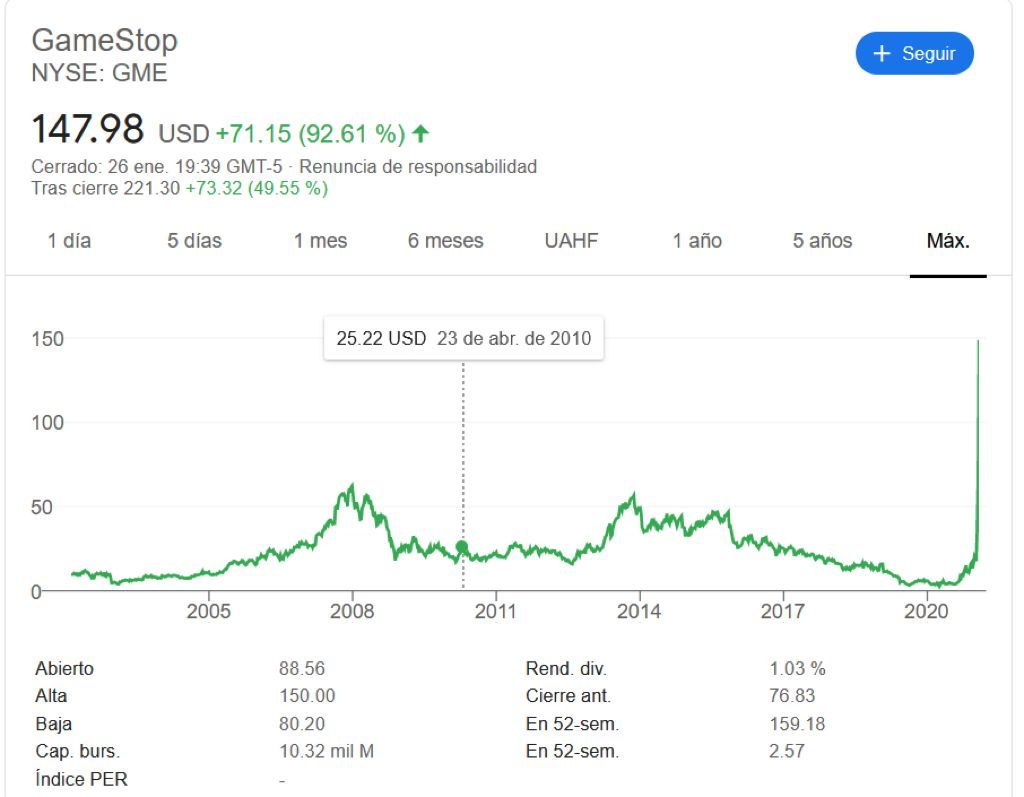
\includegraphics[width=\textwidth]{../code/figures/gamestop-stocks}
\centering
\caption{Gamestop stock from the last days}
\label{fig:gamestop-stock}
\end{figure}

Sin embargo, esta estrategia llegó a oídos de los miembros del subreddit \textit{wallstreetbets}, a quienes les pareció mal cómo se estaban comportando estos inversores. Decidieron tomar la decisión de comprar estas acciones baratas, inflando rápidamente el valor mucho más allá de lo que esperaban los administradores de fondos de cobertura, de manera que algunos miembros de Reddit han llegado a pagar miles de dólares con el objetivo de reventar los planes de los inversores mencionados anteriormente [\ref{fig:gamestop-stock}]. Mientras que \textit{wallstreetbets} celebran la locura y dicen que no van a vender y seguir comprando (incluso hay gente que compro hace año y medio una call con 50k y si la ejecuta se llevaría 36 millones ahora mismo) \cite{call}. Ahora los compradores de Reddit deben calcular cuándo vender sus acciones para obtener beneficio, el cual podría ser de hasta 3.000 veces lo que compraron. Además, están explorando otros informes de \textbf{AMC} y \textbf{BlackBerry}, una cadena de cines estadounidense y una empresa de tecnología canadiense, para llevar a cabo acciones similares. \textbf{Otro tema interesante podría ser que debido a este fenómeno hay gente aplicando análisis de opiniones/sentimientos} en este foro de reddit para ver cuál puede ser el próximo objetivo pero esto ya se sale de nuestro tema elegido que es la detección de anomalias.

Para los datos, vamos a utilizar el paquete \textit{pandas-datareader} \cite{pandas-datareader} \footnote{The Pandas datareader is a sub package that allows one to create a dataframe from various internet datasources, currently including: Yahoo! Finance. Google Finance.} donde extraeremos los datos trading volume data de Yahoo Finance. En nuestro caso, nuestras características de entrada serán una lista de símbolos ETF, los comentados anteriormente que corresponderán a Gamestop (GME), Blackberry (BB), Nokia (NOK) y AMC. Definiremos este entorno como nuestro "mercado", aunque en la práctica podríamos hacer que sea mucho, mucho más grande. Cogemos fechas desde hace 5 años hasta hoy, donde han ocurrido los acontecimientos recientes. Mostramos imagenes del trading volume y del precio de cierre en la figuras [\ref{fig:trading-volume}] y [\ref{fig:closing-price}] respectivamente.

\begin{figure}[H]
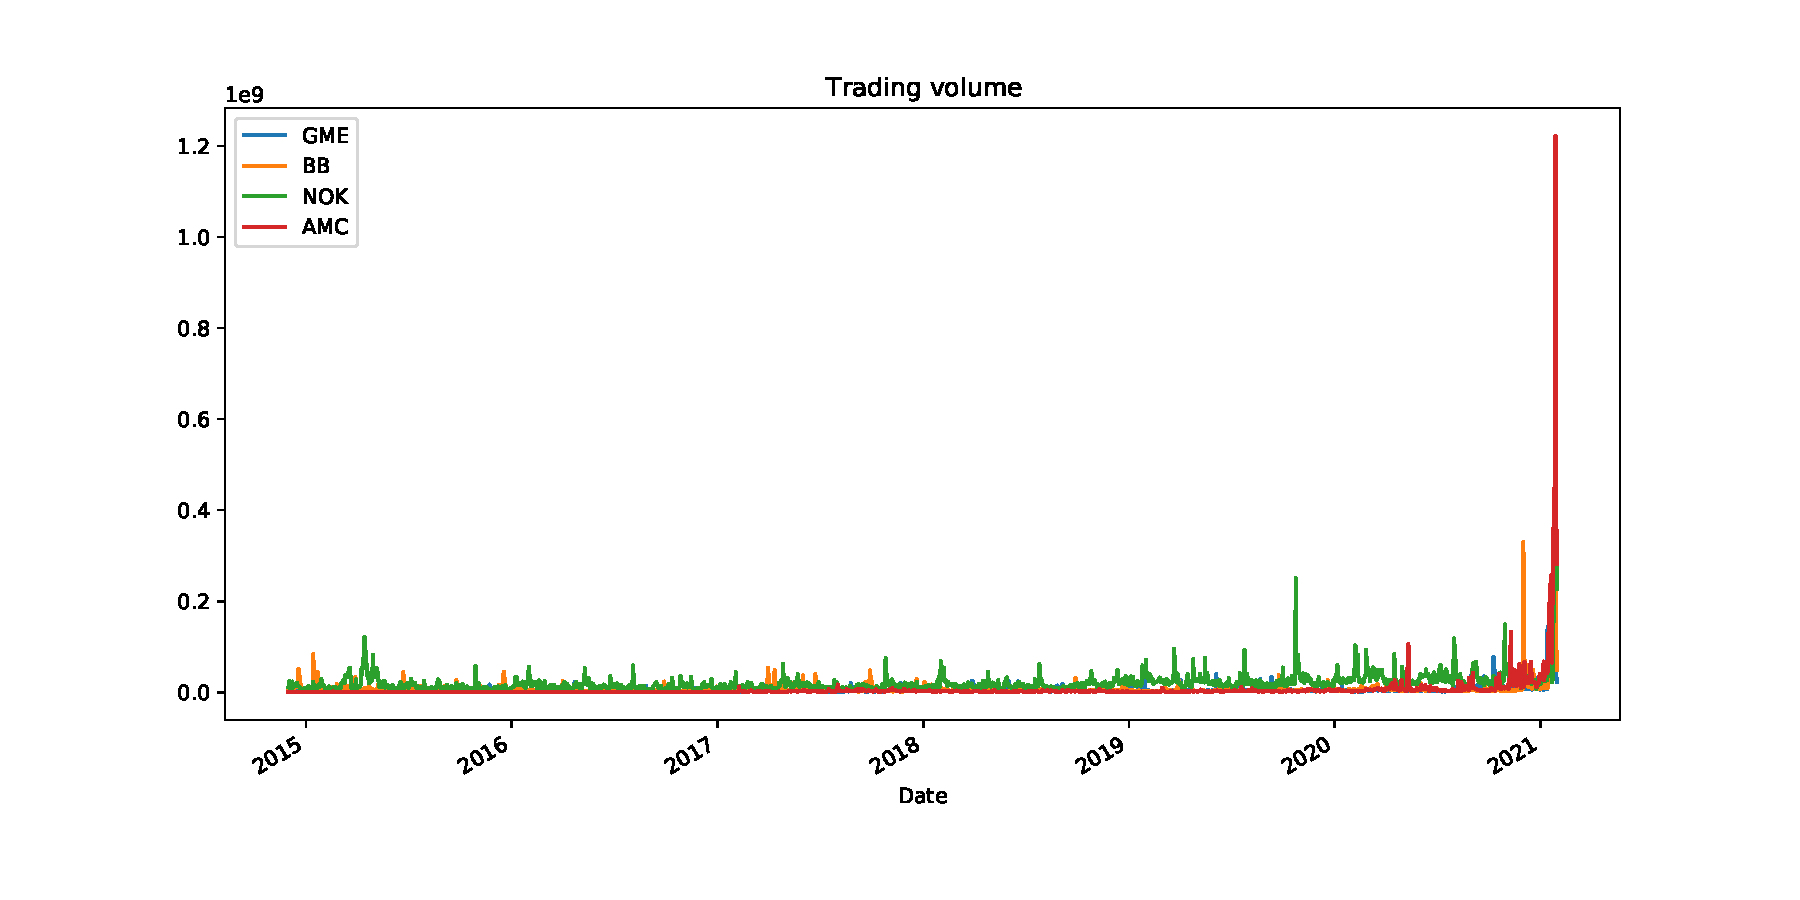
\includegraphics[width=\textwidth]{../code/figures/trading_volume.pdf}
\centering
\caption{Trading volume data}
\label{fig:trading-volume}
\end{figure}

\begin{figure}[H]
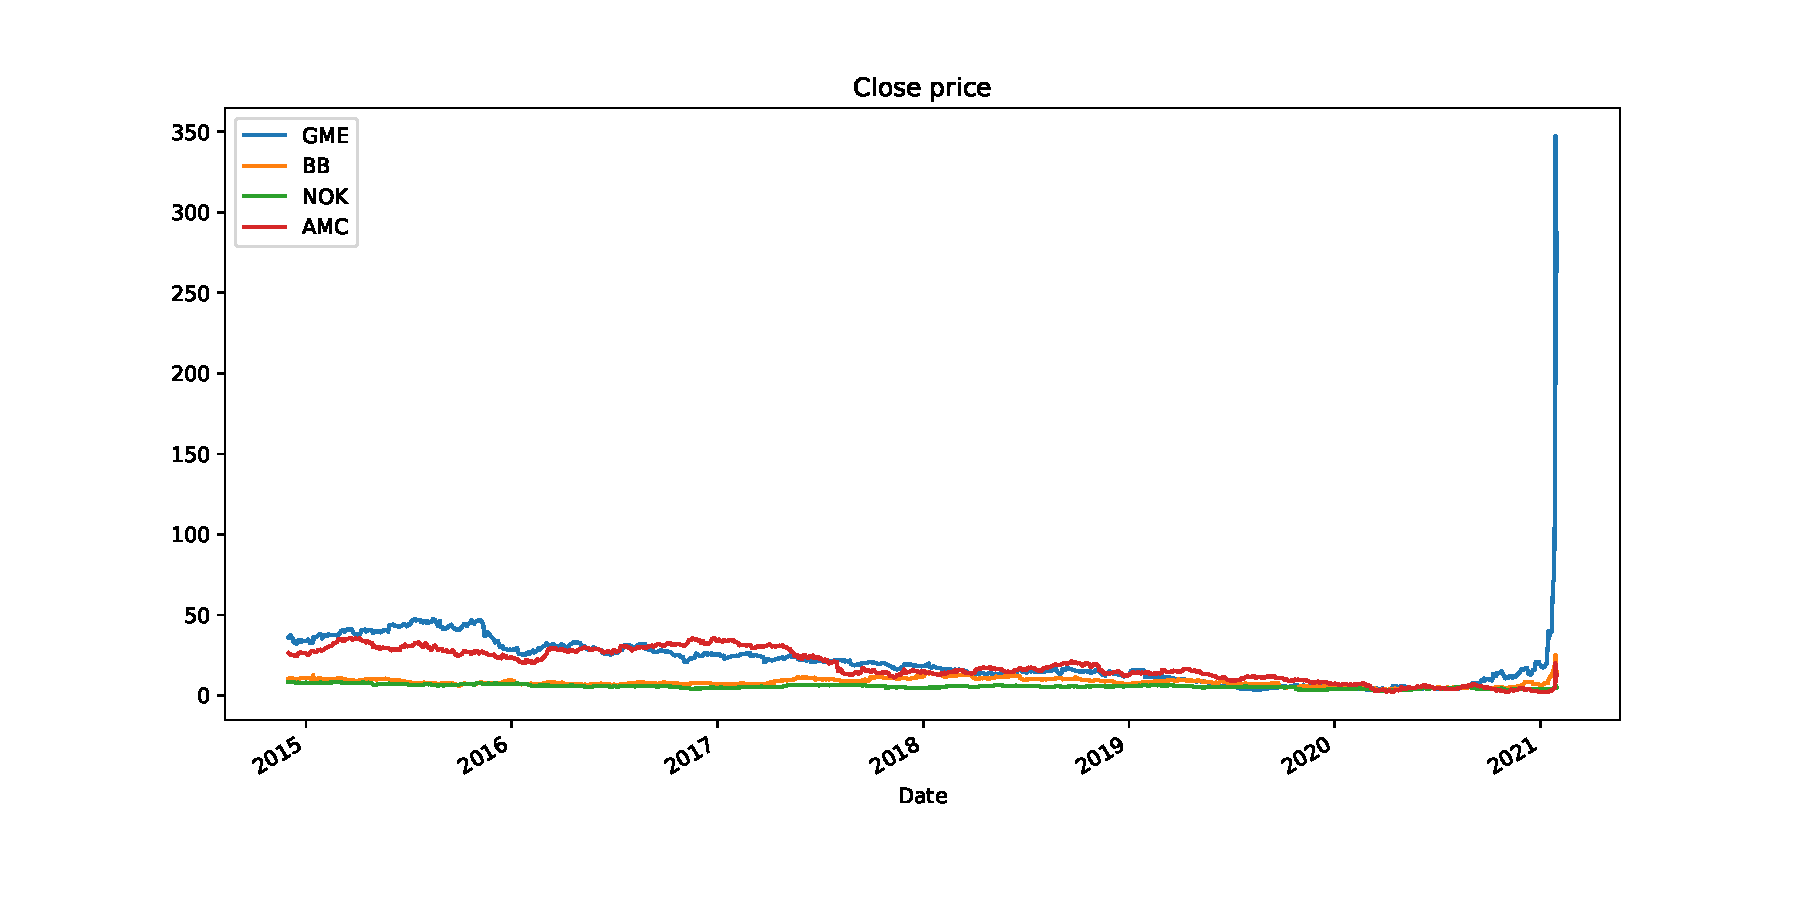
\includegraphics[width=\textwidth]{../code/figures/close_price.pdf}
\centering
\caption{Closing Price}
\label{fig:closing-price}
\end{figure}

En el comercio como en la vida, a menudo es extremadamente valioso determinar si el entorno actual es anómalo o no de alguna manera. Si las cosas están actuando "normalmente", sabemos que nuestras estrategias pueden operar de cierta manera. Por ejemplo, si nos encontramos en un entorno comercial normal, podríamos emplear una estrategia de volatilidad en corto. Por otro lado, si identificamos que estamos en un mercado anormalmente emocionante, podría ser necesario emplear una estrategia que haga exactamente lo contrario: buscar oportunidades para el comercio basado en el impulso, por ejemplo. En ese tipo de mercado, acortar la volatilidad podría ser muy peligroso. El objetivo será aplicar una serie de algoritmos para determinar cuándo el volumen de operaciones de nuestra lista de símbolos se encuentra en un estado anómalo. Esto podría significar, por ejemplo, que estamos detectando un pico en el volumen de operaciones.

%%%%%%%%%%%%%%%%%%%%%%%%%%%%%%%%%%%%
\chapter*{Descripción de los algoritmos}
\addcontentsline{toc}{chapter}{Descripción de los algoritmos}  

Vamos a utilizar y comparar algoritmos de las bibliotecas PyOD \cite{pyod} y Scikit-Learn Outlier Detection \cite{sklearn}, primero, vamos a comentar algunos de ellos. El módulo Python Outlier Detection (PyOD) facilita el modelado de detección de anomalías. Recopila una amplia gama de técnicas que van desde el aprendizaje supervisado hasta las técnicas de aprendizaje no supervisado. No es necesario probar todas las técnicas para encontrar anomalías. Dependiendo de los datos, algunas técnicas funcionan mejor que otras. Típicamente el problema de detección de anomalías es un problema no supervisado, esto quiere decir que nuestros algoritmos no tienen etiquetas para entrenar. No obstante tenemos aproximaciones de algoritmos supervisados para este tipo de problemas, aunque debido al conjunto de datos que hemos elegido donde tenemos un problema de aprendizaje no supervisado (cluster) donde intentaremos aprender el patrón de lo datos pero no mediante conjuntos de entrenaimiento sino por esta demasiado lejos de un grupo, directamente sobre el conjunto aplicamos las ténicas, luego es un problema no supervisado donde nos centraremos principalmente en algoritmos no supervisados de las librerias comentadas anterioremente. 

Los algoritmos que probaremos algoritmos no supervisados han sido escogidos de la documentación de PyOD \cite{lista} y son los siguientes:

\begin{enumerate}
	\item \textbf{Linear Models for Outlier Detection}
	\begin{enumerate}
		\item \textbf{PCA}: Principal Component Analysis es una reducción de dimensionalidad lineal que utiliza la descomposición de valores singulares
     de los datos para proyectarlo a un espacio dimensional inferior. Aunque tiene una gran cantidad de usos nosotros vamos a centrarnos en detección de anomalías.

     En este procedimiento, la matriz de covarianza de los datos se puede descomponer en
     vectores ortogonales, llamados autovectores, asociados con autovalores. los
     vectores propios con valores propios altos capturan la mayor parte de la varianza en el
     datos.

     Por lo tanto, un hiperplano de baja dimensión construido por k autovectores puede
     capturar la mayor parte de la varianza en los datos. Sin embargo, los valores atípicos son diferentes
     de puntos de datos normales, que es más obvio en el hiperplano
     construido por los autovectores con pequeños autovalores.

     Por lo tanto, los valores anomalos buscados se pueden obtener como la suma de los valores proyectados
     distancia de una muestra en todos los vectores propios y la puntuación será la suma de la distancia euclidiana ponderada entre cada muestra y la
     hiperplano construido por los autovectores seleccionados.
		\item \textbf{Minimum Covariance Determinant (MCD)} (use the mahalanobis distances as the outlier scores). Es un estimador robusto de covarianza.

     Se aplicará el estimador de covarianza determinante de covarianza mínima
     en datos distribuidos en gauss, pero aún podría ser relevante en datos
     extraído de una distribución simétrica unimodal. No está destinado a ser utilizado
     con datos multimodales (el algoritmo utilizado para ajustar un objeto MinCovDet es
     probable que falle en tal caso).
     Se deben considerar métodos de búsqueda de proyecciones para hacer frente a multimodales
     conjuntos de datos.

     Primero se ajusta un modelo determinante de covarianza mínima y luego calcule el
     Distancia de Mahalanobis como el grado atípico de los datos
		\item \textbf{One-Class Support Vector Machines (OCSVM)}. Ya hemos visto en clase este tipo de modelos, solo que en este caso se plantea otra funcionalidad. Detección de valores atípicos sin supervisión esstimando el soporte de una distribución de alta dimensión. La implementación se basa en libsvm de Sklearn aunque utilizaremos el algoritmo de PyOD.
	\end{enumerate}
	\item \textbf{Proximity-Based Outlier Detection Models}
	\begin{enumerate}
		\item \textbf{Local Outlier Factor (LOF)}
		La puntuación de anomalía de cada muestra se denomina Factor de valor atípico local (LOF).
     Mide la desviación local de densidad de una muestra dada con
     respeto a sus vecinos, es local en el sentido de que la puntuación de anomalía depende de qué tan aislado esté el objeto
     es con respecto al vecindario circundante.
     Más precisamente, la localidad está dada por k vecinos más cercanos, cuya distancia
     se utiliza para estimar la densidad local.
     Comparando la densidad local de una muestra con las densidades locales de
     sus vecinos, uno puede identificar muestras que tienen un sustancialmente menor
     densidad que sus vecinos. Estos se consideran valores atípicos.
		\item \textbf{Clustering-Based Local Outlier Factor (CBLOF)} 
		CBLOF toma como entrada el conjunto de datos y el modelo de clúster que se
     generado por un algoritmo de agrupamiento. Clasifica los grupos en pequeños
     clústeres y clústeres grandes utilizando los parámetros alfa y beta.
     Luego, la puntuación de anomalía se calcula en función del tamaño del clúster
     punto al que pertenece, así como la distancia al cúmulo grande más cercano.

     Utiliza la ponderación para el factor de valores atípicos en función de los tamaños de los grupos como
     propuesto en la publicación original. Dado que esto puede llevar a
     comportamiento (no se encuentran valores atípicos cercanos a grupos pequeños), está deshabilitado
     Las puntuaciones de Outliers se calculan únicamente en función de su distancia a
     el centro grande más cercano.

     De forma predeterminada, kMeans se utiliza para el algoritmo de agrupación en clústeres en lugar de
     Algoritmo Squeezer mencionado en el artículo original por múltiples razones.
		\item \textbf{k Nearest Neighbors  (kNN)}  De nuevo, ya hemos visto este tipo de algoritmo en la asignatura, solo que en este caso se usa la distancia al kth vecino más cercano como puntuación de anomalía.
		\item \textbf{Median kNN Outlier Detection}  Igual que antes solo que utilizando la median distance.
		\item \textbf{Histogram-based Outlier Score (HBOS)} es un algoritmo es un eficiente sin supervisión. Asume la independencia de la función y calcula el grado de las anomalías mediante la construcción de histogramas.
	\end{enumerate}
	\item \textbf{Probabilistic Models for Outlier Detection}
	\begin{enumerate}
		\item \textbf{Angle-Based Outlier Detection (ABOD)} Considera la relación entre cada punto y su (s) vecino (s). No considera las relaciones entre estos vecinos. La varianza de sus puntuaciones de coseno ponderadas a todos los vecinos podría verse como la puntuación periférica. Funciona bien en multidimensional data.
	\end{enumerate}
	\item \textbf{Outlier Ensembles and Combination Frameworks}
	\begin{enumerate}
		\item \textbf{Isolation Forest} Utiliza la biblioteca scikit-learn internamente. En este método, la partición de datos se realiza mediante un conjunto de árboles. Isolation Forest proporciona una puntuación de anomalía al observar qué tan aislado está el punto en la estructura. Luego, la puntuación de anomalía se utiliza para identificar valores atípicos de observaciones normales
Isolation Forest funciona bien en datos multidimensionales
		\item \textbf{LSCP} LSCP es un conjunto de detección de valores atípicos paralelo no supervisado que selecciona
    detectores competentes en la región local de una instancia de prueba. Esta
    La implementación utiliza una estrategia de Promedio de Máximo \textit{(Average of Maximum)}. Primero, un heterogéneo
    La lista de detectores base se ajusta a los datos de entrenamiento y luego genera un
    la verdad pseudo-terrestre para cada instancia de tren es generada por
    tomando la puntuación máxima de valores atípicos.

    Para cada instancia de prueba:
    	\begin{enumerate}
       \item La región local se define como el conjunto de puntos de entrenamiento más cercanos en
    subespacios de características muestreados aleatoriamente que ocurren con más frecuencia que
    un umbral definido en múltiples iteraciones.

    \item Usando la región local, se define una verdad de pseudo terreno local y la
    La correlación de pearson se calcula entre el entrenamiento de cada detector base
    puntajes atípicos y la verdad pseudo fundamental.

\item Se construye un histograma a partir de las puntuaciones de correlación de Pearson; detectores en
    los contenedores más grandes se seleccionan como detectores de base competentes para el
    instancia de prueba.

    \item Se toma la puntuación promedio de valores atípicos de los detectores competentes seleccionados
    para ser la puntuación final.
    	\end{enumerate}
	\end{enumerate}
\end{enumerate}


\chapter*{Estudio experimental}
\addcontentsline{toc}{chapter}{Estudio experimental}  

\textcolor{blue}{Todo lo relacionado con esta parte de la práctica puede encontrarse en mi repositorio de \textbf{\href{https://github.com/daviduster/anomaly-detection-stock}{github}}}.\\
\\

Vamos a proceder a aplicar los algoritmos anteriores con los datos comentado en la descripción del problema, en las figuras [\ref{fig:trading-volume}] y [\ref{fig:closing-price}]. Inicialmente hagamos un describe para ver los datos en la tabla [\ref{tab:describe}]

\begin{table}[H]
\centering
\begin{tabular}{lrrrr}
\toprule
{} &           GME &            BB &           NOK &           AMC \\
\midrule
count &  1.047000e+03 &  1.047000e+03 &  1.047000e+03 &  1.047000e+03 \\
mean  &  5.781856e+06 &  7.729197e+06 &  2.394326e+07 &  8.067518e+06 \\
std   &  1.296132e+07 &  2.352192e+07 &  4.480880e+07 &  4.861418e+07 \\
min   &  9.729000e+05 &  1.054900e+06 &  3.136300e+06 &  1.802000e+05 \\
25\%   &  2.257900e+06 &  2.954850e+06 &  1.197440e+07 &  1.430500e+06 \\
50\%   &  3.215900e+06 &  3.960900e+06 &  1.817230e+07 &  2.155200e+06 \\
75\%   &  5.204550e+06 &  6.122550e+06 &  2.613805e+07 &  3.928200e+06 \\
max   &  1.967843e+08 &  3.722226e+08 &  1.123003e+09 &  1.222342e+09 \\
\bottomrule
\end{tabular}
\caption{Describe}
\label{tab:describe}
\end{table}

El campo es bastante complejo, a priori nuestro dataset depende del tiempo, en general los datos financieros son procesos estocásticos ya que tenemos la variable del tiempo, al obviar el factor del tiempo no estamos teniendo en cuenta algo muy importante, también habría que ver que definimos con un pico u outlier, una subida muy alta de la cotización de los retornos? Puede que este tipo de cosas sea cíclicas y normales respecto a la serie del tiempo. Para facilitar el tema elegido simplemente aplicaremos los algoritmos sobre un atributo o sobre ambos para facilitar la comparación y visualización y comentar los resultados. 

En general nuestra serie temporal de volumen tiene picos significativos en el volumen de operaciones en nuestros ETF elegidos. Algunos eventos notables incluyen la caída repentina del Tesoro de octubre de 2014, el aumento de la volatilidad en agosto de 2015, así como la elección de Donald Trump a fines de 2016. Nótese la relativa calma a principios de 2017 ...

Si bien estos eventos son obvios a simple vista (mucho después del hecho), lo que sería útil es la capacidad de clasificar automáticamente los eventos basándose únicamente en los datos del volumen de operaciones, es decir, sin el uso de un ser humano. Este es el objetivo del aprendizaje automático y, afortunadamente, este es exactamente el tipo de caso de uso para utilizar nuestros algoritmo.

Inicialmente creo que es necesario trabajar con un ejemplo simple de método de detección de anomalías con una variable únicamente en el que detectamos valores atípicos a partir de una distribución de valores en un solo espacio de características. Por ello, utilizaremos únicamente los datos del atributo de \textbf{Gamestop(GME)} y vamos a encontrar patrones en volumen de trading y closing price por separado que no se ajustan al comportamiento esperado. Es decir, detectar valores atípicos para una variable a la vez.

Mostramos una pequeña visualizión inicial de nuestro conjunto de datos.

\begin{lstlisting}
Skewness: 10.093959
Kurtosis: 122.632442
\end{lstlisting}

En las imagenes [\ref{fig:dist-trading-GME}] y [\ref{fig:dist-closing-GME}] vemos que está lejos de una distribución normal, y tiene una cola larga y delgada positiva, la masa de la distribución se concentra a la izquierda de la figura. Las distribuciónes superan con creces las colas de la distribución normal.
Hay una región donde los datos tienen baja probabilidad de aparecer y está en el lado derecho de la distribución.

\begin{figure}[H]
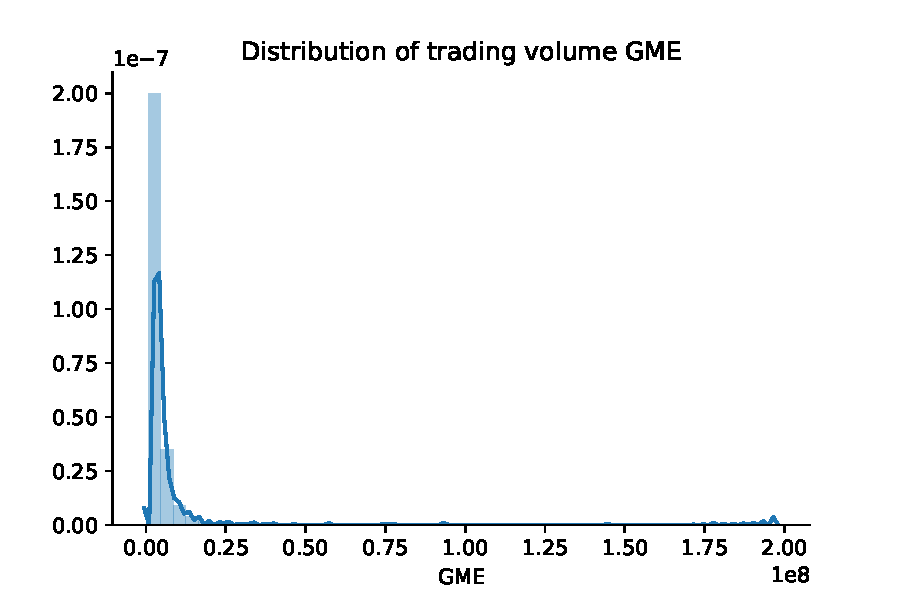
\includegraphics[width=\textwidth]{../code/figures/distribution_trading_volume_GME.pdf}
\centering
\caption{Distribución trading volume GME}
\label{fig:dist-trading-GME}
\end{figure}

\begin{figure}[H]
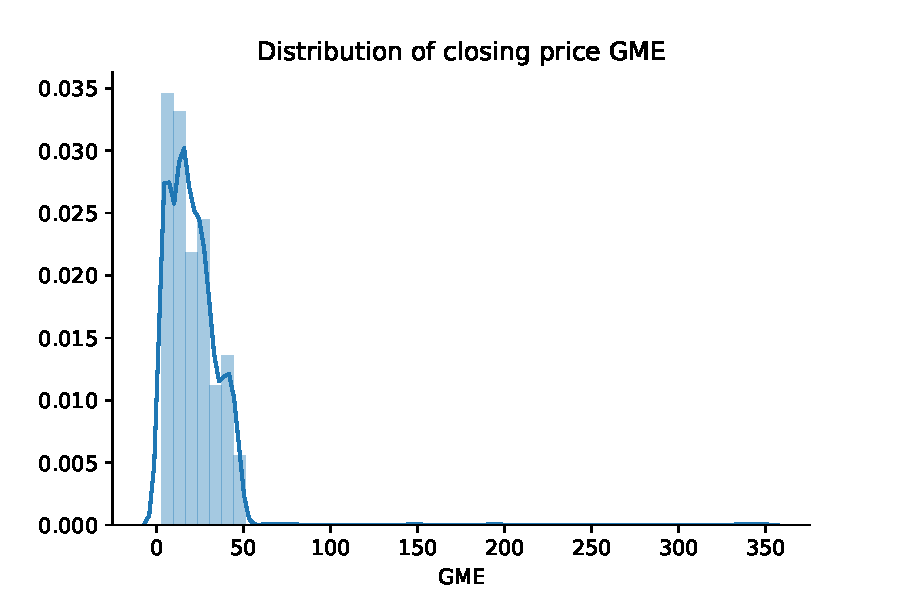
\includegraphics[width=\textwidth]{../code/figures/distribution_closing_price_GME.pdf}
\centering
\caption{Distribución closing price GME}
\label{fig:dist-closing-GME}
\end{figure}

Como hemos visto antes, Isolation Forest es un algoritmo para detectar valores atípicos que devuelve la puntuación de anomalía de cada muestra utilizando el algoritmo IsolationForest que se basa en el hecho de que las anomalías son puntos de datos que son pocos y diferentes. Isolation Forest es un modelo basado en árboles. En estos árboles, las particiones se crean seleccionando primero al azar una característica y luego seleccionando un valor de división aleatoria entre el valor mínimo y máximo de la característica seleccionada. Vamos a utilizar este algoritmo que funciona para Univariate Anomaly Detection en el caso de GME. 

El siguiente proceso muestra cómo se comporta IsolationForest en el caso de GME,
IsolationForest entrenado usando los datos de GME. Almacenamos el valor en una matriz NumPy para usarla en nuestro modelo más adelante. Calcula la puntuación de anomalía para cada observación. La puntuación de anomalía de una muestra de entrada se calcula como la puntuación media de anomalía de los árboles en el bosque. Clasificamos cada observación como un valor atípico o no atípico. Y finalmente usamos visualización para resaltar las regiones donde caen los valores atípicos.

\begin{figure}[H]
\begin{multicols}{2}
    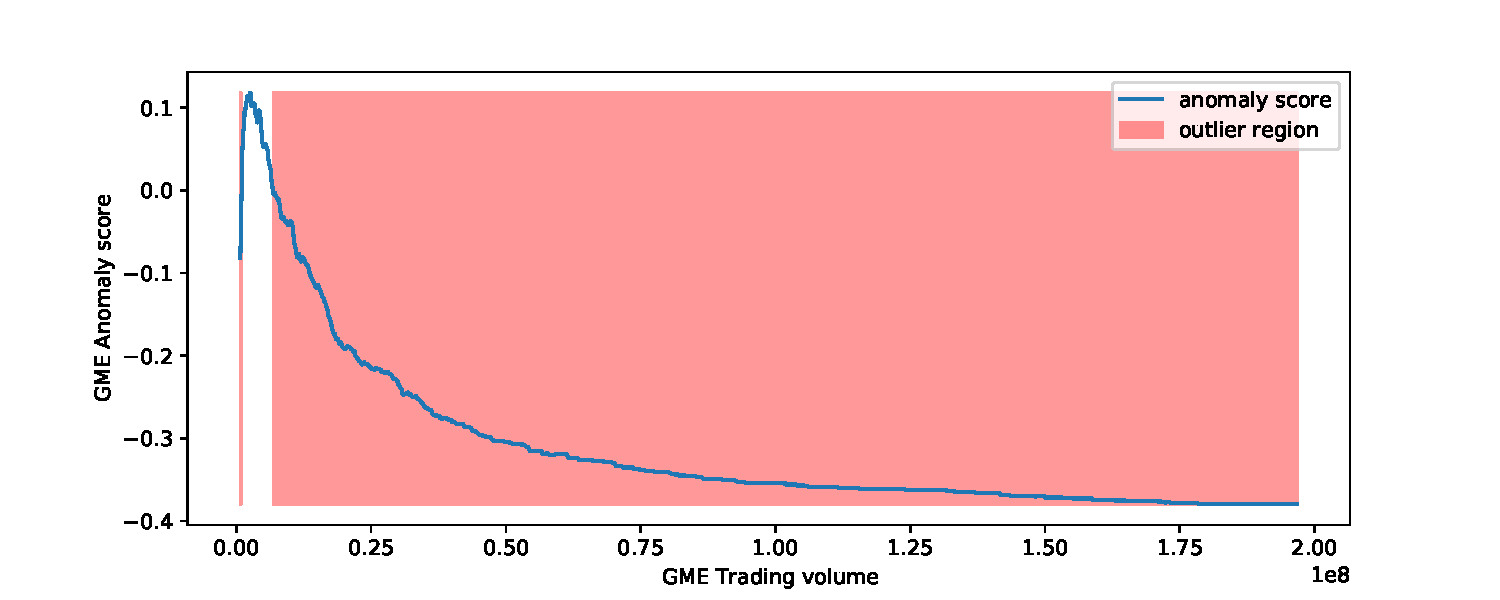
\includegraphics[width=9cm]{../code/figures/if_trading_GME.pdf}\par 
    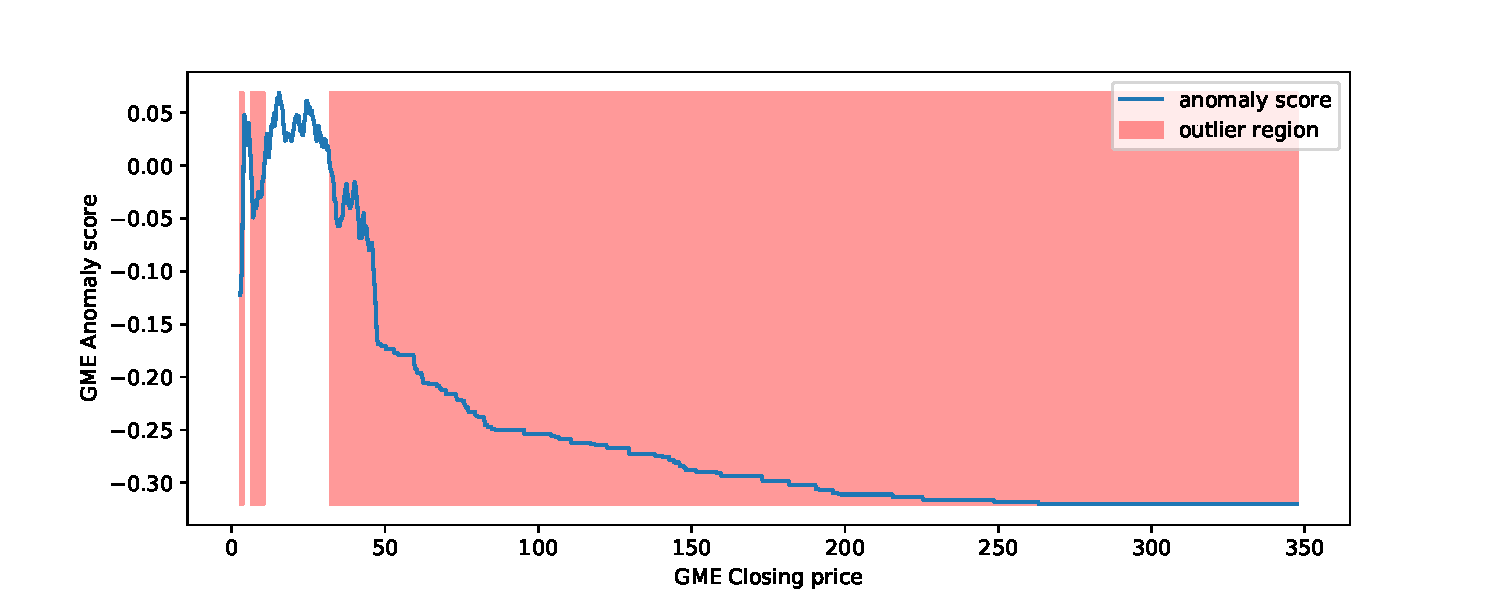
\includegraphics[width=9cm]{../code/figures/if_closing_GME.pdf}\par 
\end{multicols}
\caption{Isolation Forest GME}
\label{fig:if-GME}
\end{figure}

\begin{figure}[H]
\begin{multicols}{2}
    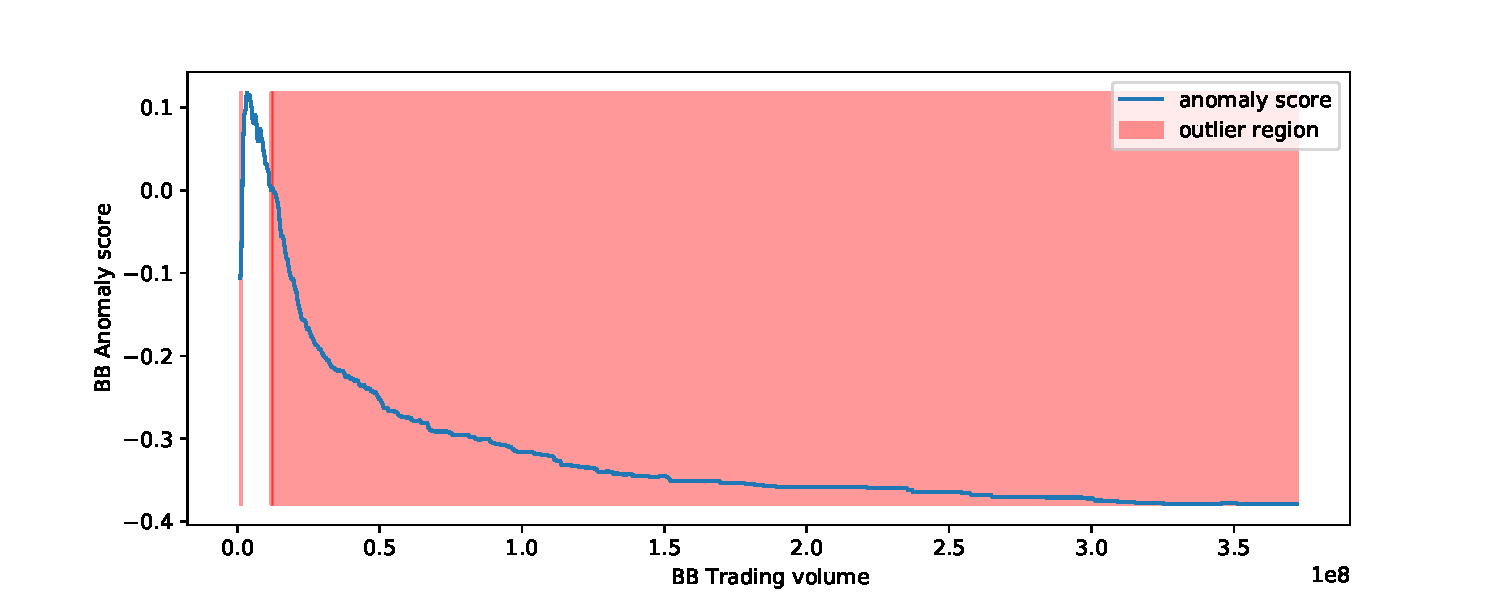
\includegraphics[width=9cm]{../code/figures/if_trading_BB.pdf}\par 
    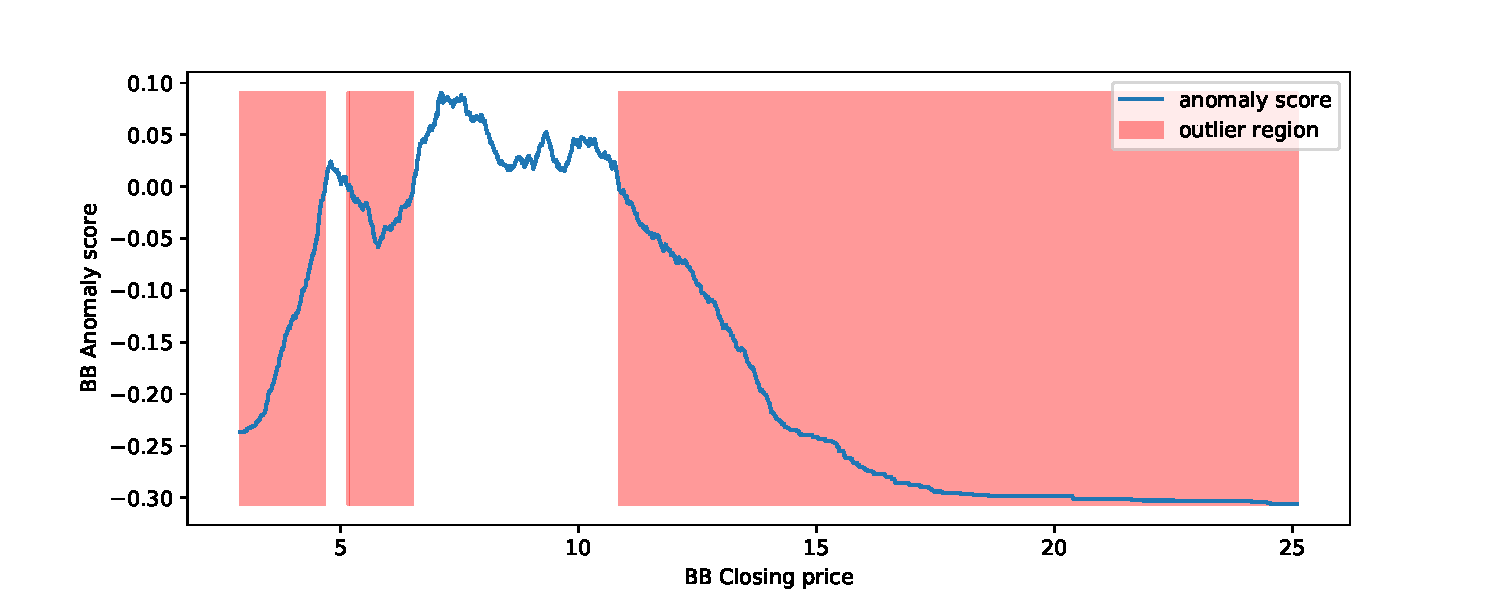
\includegraphics[width=9cm]{../code/figures/if_closing_BB.pdf}\par 
\end{multicols}
\caption{Isolation Forest BB}
\end{figure}

\begin{figure}[H]
\begin{multicols}{2}
    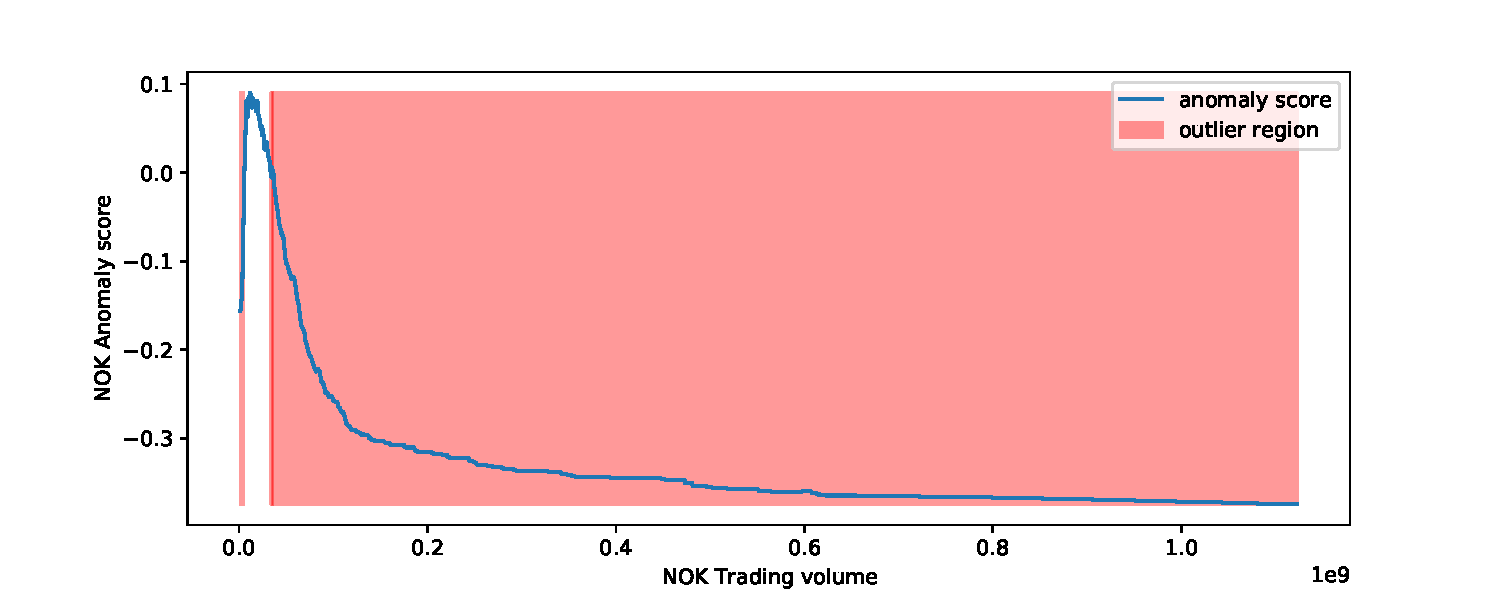
\includegraphics[width=9cm]{../code/figures/if_trading_NOK.pdf}\par 
    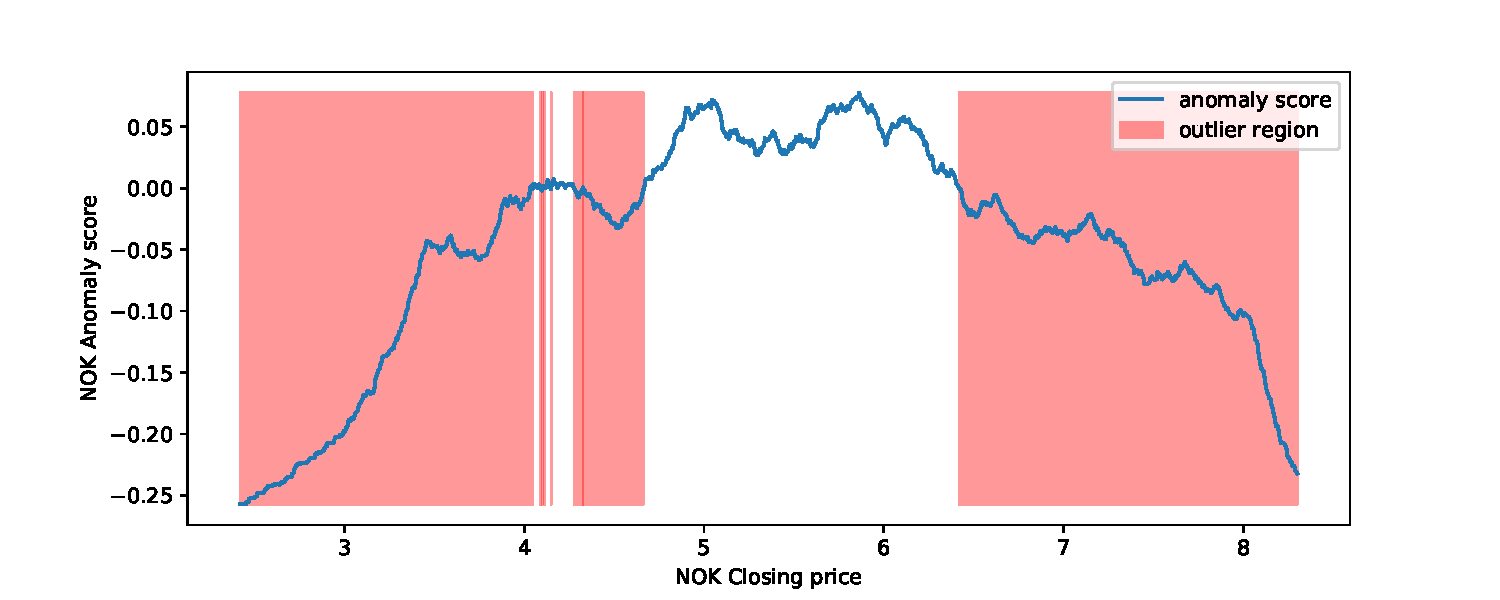
\includegraphics[width=9cm]{../code/figures/if_closing_NOK.pdf}\par 
\end{multicols}
\caption{Isolation Forest NOK}
\end{figure}

\begin{figure}[H]
\begin{multicols}{2}
    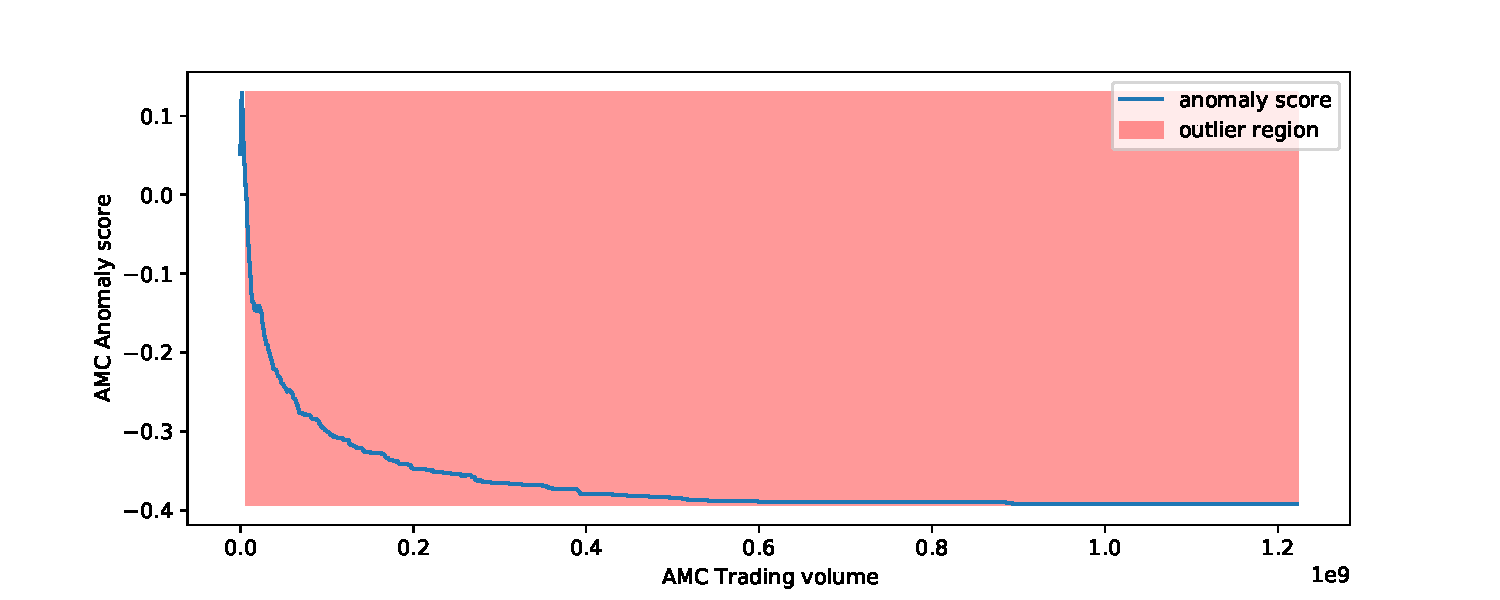
\includegraphics[width=9cm]{../code/figures/if_trading_AMC.pdf}\par 
    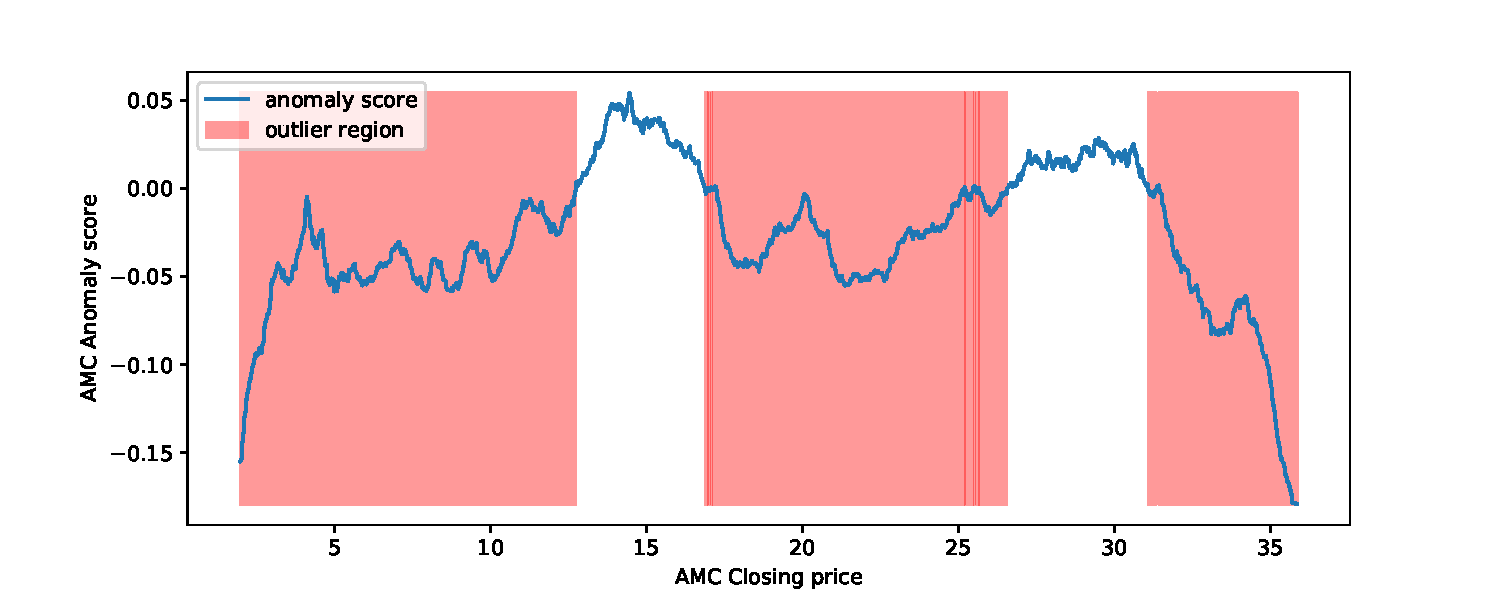
\includegraphics[width=9cm]{../code/figures/if_closing_AMC.pdf}\par 
\end{multicols}
\caption{Isolation Forest AMC}
\label{fig:if-AMC}
\end{figure}


En las imagenes de la izquiera tenemos la visualización del algoritmo  con respecto el trading volume, y a la derecha respecto al closing price. Una puntuación cercana a 1 indica anomalías. Una puntuación mucho menor que 0,5 indica observaciones normales. Si todas las puntuaciones se acercan a 0,5, entonces la muestra completa no parece tener anomalías claramente diferenciadas. Por ejemplo, en la figura de la izquierda de [\ref{fig:if-GME}], valores por encima de 0,15 definitivamente se considera un outlier. Lo cual concuerda visualmente con la gráfica [\ref{fig:trading-volume}]. Al contrario que la imagen de la derecha donde comparado con la gráfica de la izquierda, los resultados y la visualización anteriores, parece que los beneficios que estén fuera del intervalo blanco se considerarían un valor atípico, lo cuál visualmente tiene sentido. De igual manera razonaríamos para los demás casos. Destacamos [\ref{fig:if-AMC}] donde al ser más estable la gráfica, es normal que cualquier valor que sobresalga se considere un outlier.

Nuestro modelo determinó que este periodo con una gran cantidad de trading es una anomalía. Las visualizaciones anteriores muestran las puntuaciones de anomalías y resaltan las regiones donde se encuentran los valores atípicos. Como era de esperar, la puntuación de anomalía refleja la forma de la distribución subyacente y las regiones atípicas corresponden a áreas de baja probabilidad.
Sin embargo, el análisis univariante solo puede llevarnos hasta aquí. Podemos darnos cuenta de que algunas de estas anomalías determinadas por nuestros modelos no son las anomalías que esperábamos. Cuando nuestros datos son multidimensionales en lugar de univariados, los enfoques para la detección de anomalías se vuelven más intensivos desde el punto de vista computacional y más complejos matemáticamente.

La mayoría de los análisis que terminamos haciendo son multivariados debido a la complejidad del mundo en el que vivimos. En la detección de anomalías multivariadas, el valor atípico es una puntuación inusual combinada en al menos dos variables.
Entonces, usando los atributos en pares , por ejemplo GME Y BB, vamos a construir un método de detección de anomalías multivariante no supervisado basado en todos los modelos comentados anteriormente.

\begin{figure}[H]
\begin{multicols}{2}
    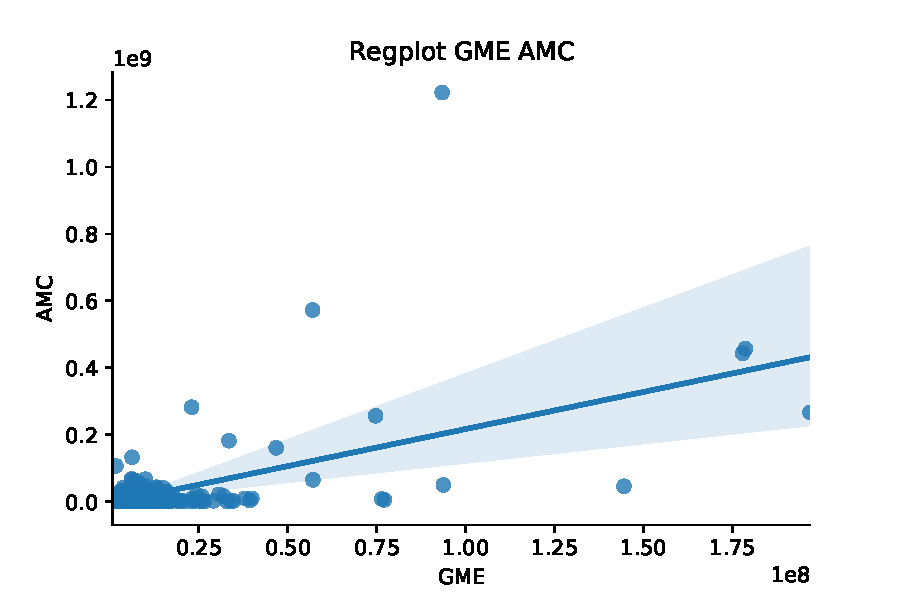
\includegraphics[width=9cm]{../code/figures/regplot_GME_AMC.pdf}\par 
    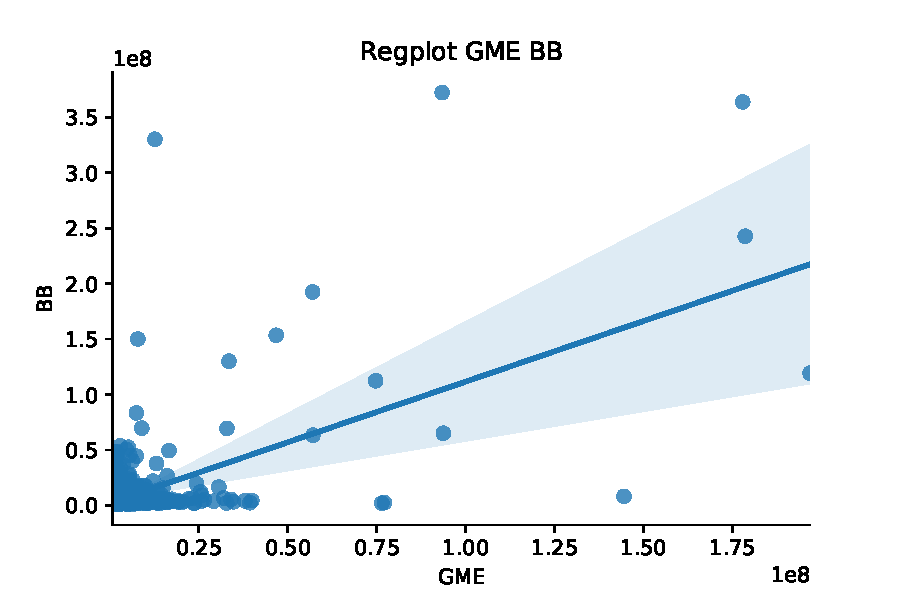
\includegraphics[width=9cm]{../code/figures/regplot_GME_BB.pdf}\par 
\end{multicols}
\caption{Regplot GME, AMC y BB}
\label{fig:regplot-1}
\end{figure}

\begin{figure}[H]
\begin{multicols}{2}
    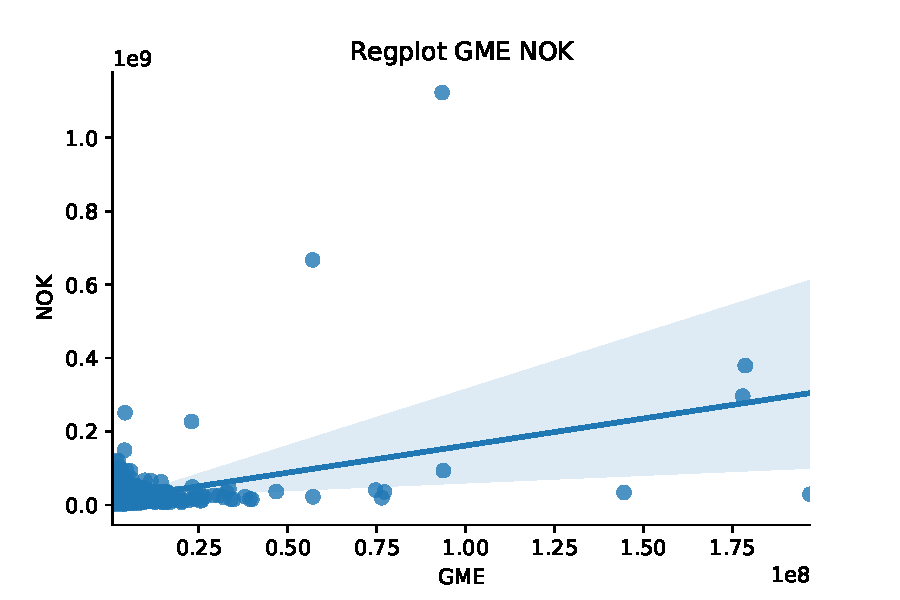
\includegraphics[width=9cm]{../code/figures/regplot_GME_NOK.pdf}\par 
    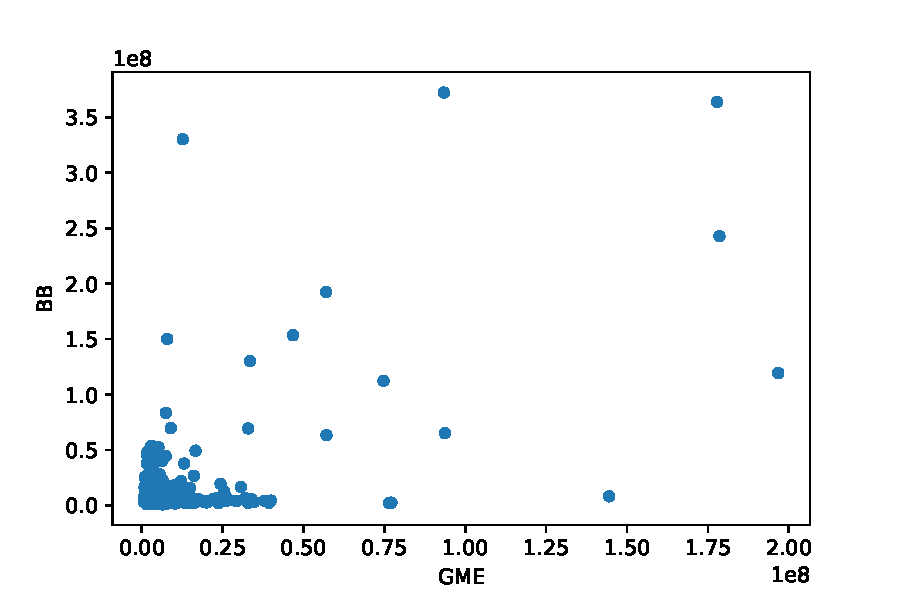
\includegraphics[width=9cm]{../code/figures/GME_BB.pdf}\par 
\end{multicols}
\caption{Regplot GME y Nokia y Scatter plot GME y BB}
\label{fig:regplot-2}
\end{figure}

\begin{figure}[H]
\begin{multicols}{2}
    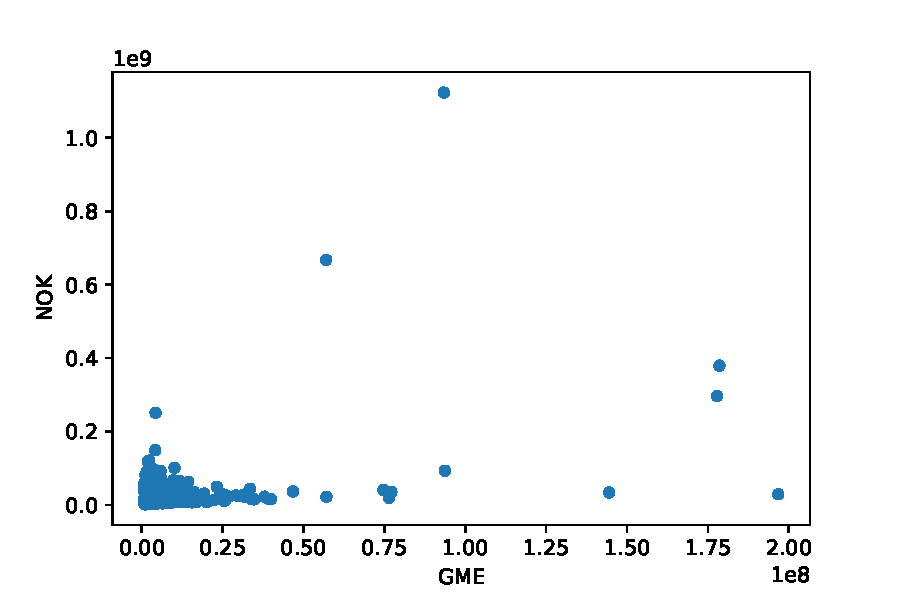
\includegraphics[width=9cm]{../code/figures/GME_NOK.pdf}\par 
    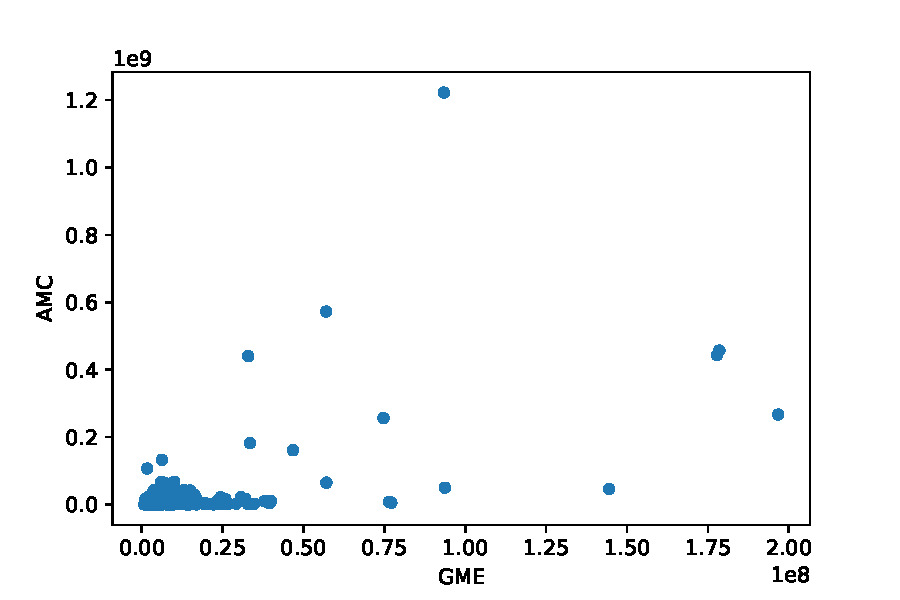
\includegraphics[width=9cm]{../code/figures/GME_AMC.pdf}\par 
\end{multicols}
\caption{Regplot GME y Nokia y Scatter plot GME y BB}
\label{fig:regplot-3}
\end{figure}


\chapter*{Planteamiento de futuro}
\addcontentsline{toc}{chapter}{Planteamiento de futuro}  


%% bibliography
\medskip

\printbibliography[
heading=bibintoc,
title={Referencias}
]


\end{document}
